\documentclass{chi2009}
\usepackage{times}
\usepackage{url}
\usepackage{graphics}
\usepackage{color}
\usepackage[pdftex]{hyperref}
\hypersetup{%
pdftitle={TwinList: \\ Visualizing List Differences},
pdfauthor={Leonardo Max Baptista Claudino, claudino@cs.umd.edu \\
	    Sameh Khamis, sameh@cs.umd.edu \\
	    Ran Liu, ranliu@cs.umd.edu \\
	    Ben London, blondon@cs.umd.edu \\
	    Jay Pujara, jay@cs.umd.edu},
pdfkeywords={list visualization},
bookmarksnumbered,
pdfstartview={FitH},
colorlinks,
citecolor=black,
filecolor=black,
linkcolor=black,
urlcolor=black,
breaklinks=true,
}
\newcommand{\comment}[1]{}
\definecolor{Orange}{rgb}{1,0.5,0}
\newcommand{\todo}[1]{\textsf{\textbf{\textcolor{Orange}{[[#1]]}}}}

% TwinList Macros
\newcommand{\TwinList}{\textsc{TwinList}}
\newcommand{\ListViewer}{\textit{List Viewer}}
\newcommand{\AcceptReject}{\textit{Accept/Reject}}
\newcommand{\AcceptedRejected}{\textit{Accepted/Rejected}}
\newcommand{\Details}{\textit{Details Panel}}
\newcommand{\Tools}{\textit{Tools Dock}}
\newcommand{\Controls}{\textit{Control Panel}}
\newcommand{\Filters}{\textit{Filter Panel}}
\newcommand{\Options}{\textit{Options Panel}}
\newcommand{\SizeBy}{\textit{Size By}}
\newcommand{\ColorBy}{\textit{Color By}}
\newcommand{\GroupBy}{\textit{Group By}}
\newcommand{\SortBy}{\textit{Sort By}}
\newcommand{\Similar}{\textit{Similar}}
\newcommand{\Identical}{\textit{Identical}}
\newcommand{\Unique}{\textit{Unique}}

\pagenumbering{arabic}  % Arabic page numbers for submission.  Remove this line to eliminate page numbers for the camera ready copy

\begin{document}
% to make various LaTeX processors do the right thing with page size
\special{papersize=8.5in,11in}
\setlength{\paperheight}{11in}
\setlength{\paperwidth}{8.5in}
\setlength{\pdfpageheight}{\paperheight}
\setlength{\pdfpagewidth}{\paperwidth}

% use this command to override the default ACM copyright statement 
% (e.g. for preprints). Remove for camera ready copy.
\toappear{Submitted for CMSC 734 Information Visualization.}

\title{TwinList: \\ Visualizing List Differences}
\numberofauthors{5}
\author{
  \alignauthor Leonardo Claudino \\
    \affaddr{Dept. of Computer Science, University of Maryland}\\
    \affaddr{College Park, MD 20742}\\
    \email{claudino@cs.umd.edu}
  \and
  \alignauthor Sameh Khamis\\
    \affaddr{Dept. of Computer Science, University of Maryland}\\
    \affaddr{College Park, MD 20742}\\
    \email{sameh@cs.umd.edu}
  \and
  \alignauthor Ran Liu \\
    \affaddr{Dept. of Computer Science, University of Maryland}\\
    \affaddr{College Park, MD 20742}\\
    \email{ranliu@cs.umd.edu}
  \and
  \alignauthor Ben London \\
    \affaddr{Dept. of Computer Science, University of Maryland}\\
    \affaddr{College Park, MD 20742}\\
    \email{blondon@cs.umd.edu}
  \and
  \alignauthor Jay Pujara \\
    \affaddr{Dept. of Computer Science, University of Maryland}\\
    \affaddr{College Park, MD 20742}\\
    \email{jay@cs.umd.edu}
}

\maketitle

\begin{abstract}
We present a novel list visualization tool named \TwinList, for the purpose of list visualization and matching. Leveraging Adobe's Flex platform and the Prefuse Flare toolbox, we created a rich internet application (RIA) with dynamic animated effects. These animated transitions lead the user through the procedure of matching two lists, using color coding to highlight the similarities and differences between the two. List items can be grouped, sorted and filtered according to their attribute values, to enhance workflow. To illustrate the efficacy of the application, we conduct usability testing for different applications with several domain experts and peers.
\end{abstract}

\keywords{list visualization} 

\category{H.5.2}{Information Interfaces and Presentation}{Miscellaneous}

\section{Introduction}
A common task is comparing information from different sources or about different entities. This problem occurs in everyday life as well as in specialized applications. For example, a consumer interested in making a purchase may wish to compare the features of two products. A newspaper may wish to compare the words used by different political parties during campaign speeches. Or as a more specialized example, a doctor performs the task of medical reconciliation. In medical reconciliation, a doctor crafting a treatment plan for a patient prior to their discharge from a hospital will need to compare medications the patient was taking before admission with the medications administered during hospitalization. 

A core problem shared by these applications is that data is in the form of two lists, and a decision is reached by comparing the constituent items of these lists in a structured way. One element of the list structure is that items have some similarity or correspondence between lists. The logic necessary to compare these items can be complicated, such as resolving a prescription drug and its generic equivalent as the same item in two different lists. Each item may have attributes that must be taken into consideration when assessing similarity, such as the dosage of a medication prescribed. Attributes may also be used to segment list items into categories, such as different classes of drugs. Finally, list comparison should help reach a conclusion, such as a purchasing decision or a final list of medications to prescribe a patient.

Our goal was to design a visualization that allows users to quickly answer the dual questions ``What is the same between these two lists?'' and ``What is different between these two lists?'', quickly, accurately and effortlessly. We address these aspects of the list comparison problem in our visualization tool, \TwinList. Using a spatial organization of data, we provide an intuitive way for users to quickly differentiate between items that are the same and those that differ in two lists of data. We abstract complicated similarity logic by categorizing items as ``identical'' when they are the same in both lists, ``unique'' when they appear in only one lists, and ``similar'' when the same item has different attributes in each list. We map these three categories to a workflow and use animation to help users understand each step of the list comparison process. In addition, \TwinList~ provides sorting, filtering, and grouping functionality to allow users to explore different aspects of the data. Finally, the application supports choosing items that are relevant or irrelevant, helping users reach a strong conclusion. 

\subsection{Related Work}
The specific problem of list comparison as we have framed has relatively little research. Research in areas such as visualizing text corpora and set membership have resulted in relevant work that provided a basis for extending visualization techniques to novel problem areas.  Collins et al.\cite{collins2009parallel} use tag clouds drawn from text to compare several lists, using size to indicate frequency and giving a good overview of each document. Subsequent work also extends this approach to use spatial positioning to make it easier to find unique values\cite{conwaytuscon11}. One drawback of such approaches is that they are less relevant when comparing specific list items, particularly when attributes are important for comparison. Another approach that is well-studied is the comparison of sets of data. For example, Venn Diagrams have long been used to show areas of similarity and difference, and provide a way to query for a specific group of similarities and differences\cite{kestler2005generalized}. While we prototyped a solution using Venn Diagrams, they ultimately did not fulfil all the needs of our target applications. Work on animation and attribute navigation provided inspiration to our approach as well. Chevalier et al. \cite{diffmation10} use animation and highlighting to show differences between different document revisions, which draws visual attention to differences between documents. Approaches to show and quickly navigate through list attributes, such as \cite{Chimera:1992:VBI:142750.142817} and \cite{Masui98lensbar} were part of our initial designs, but did not solve the core problem of list comparison.

\section{TwinList}
\TwinList~ is a novel list visualization tool for the purpose of illustrating the similarities and differences between two lists. It can be used in many cases where the comparison of two lists of items is required. The primary application that \TwinList~ supports is that of medication list reconciliation: comparing and reconciling multiple medications that have been prescribed to a patient from multiple sources\cite{JCAHO-2006}. However, \TwinList~ is equally adept in other applications, such as comparing bag-of-words lists or visualizing gene activity in different types of human tissue, such as normal brain tissue and brain tumor tissue.

\TwinList's interface consists of four major components: the \ListViewer, \Tools, \AcceptedRejected~ lists and \Details, as shown in (Figure~\ref{fig:interface}). The \ListViewer, located in the upper left corner of the interface, is where the list matching visualization will be performed. The initialized view displays two separated lists loaded from XML files. The \Tools, in the upper right corner, displays the \Controls, \Options~ and \Filters, which can be made visible one at a time by selecting the appropriate tab. If an item in the \ListViewer~ is selected, its detail information will be shown in the \Details~ in the lower right corner. \TwinList~ is not merely meant for visualization; it also allows users to take action. List items can be accepted or rejected, whereupon they will appear in the \AcceptedRejected~ lists.

\begin{figure*}
\begin{center}
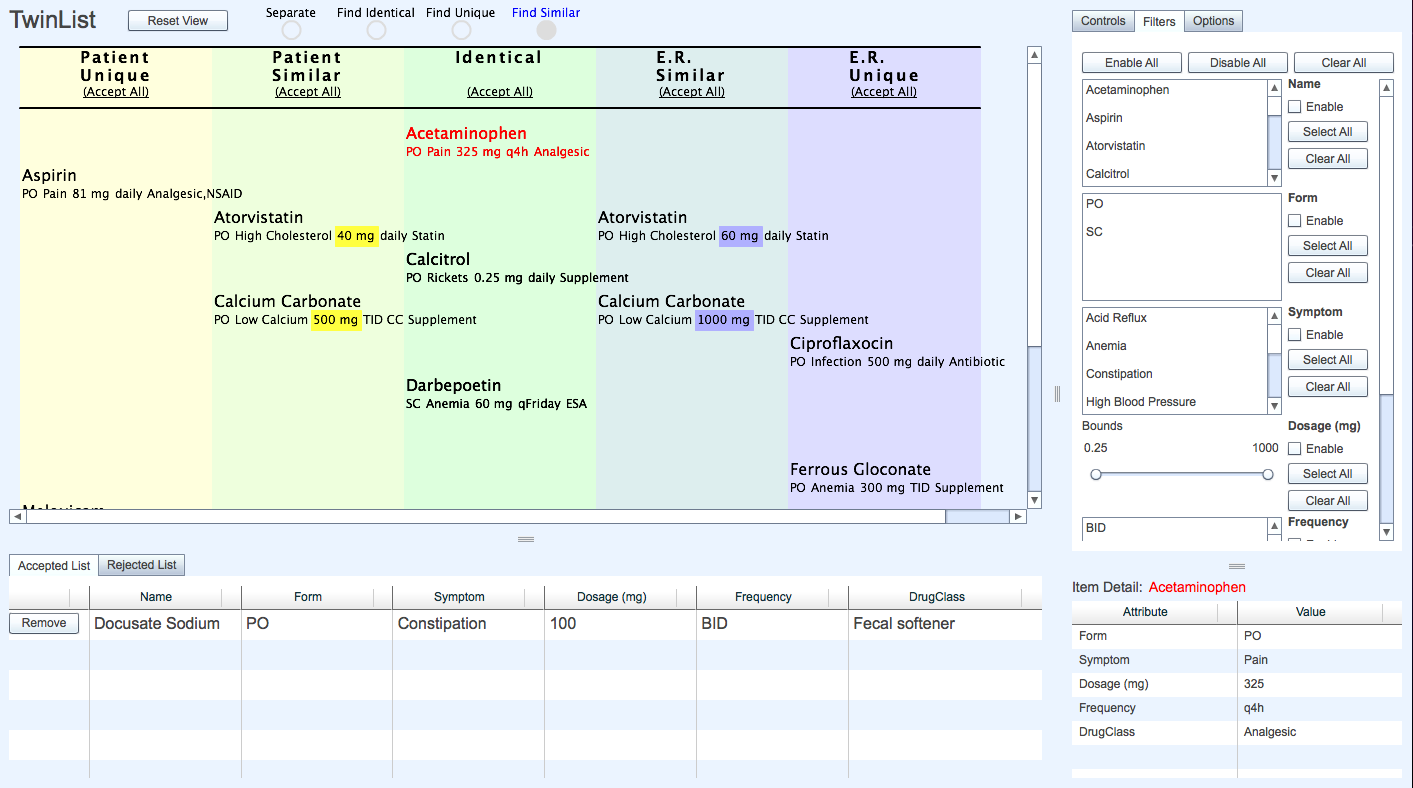
\includegraphics[width=1\linewidth]{img/interface2.png}
\end{center}
   \caption{The \TwinList~ interface: In this screen capture, the lists have been matched, displaying identical items in the center column, unique items in the outer columns and similar items in between. Color highlighting is used to indicate similar attribute values. In the bottom left panel is the \textit{Accepted} list; in the upper right panel, the \Filters; and in the lower right, the \Details, which displays all attributes for the selected item (highlighted in red).}
   \label{fig:interface}
\end{figure*}

\subsection{ListViewer}
 
\subsubsection{The five-column list placement}
To visualize the and similarity and difference of two lists, a five-column list placement is used in \TwinList. We used a different color tone to separate the two lists. That is, the items in the yellowish color columns are belong to the first list, while the ones in bluish columns are belong to the other list. 

The identical items, both the name and attributes are the same, will be shown in the center column(green). The unique items that only appeared in the first list will be shown in the leftmost column(yellow). The items that are unique to the other list then will be shown in the rightmost column (slate blue). Then all the similar items will be placed in the Similar columns and the difference will be highlighted in the visualization. For example, in Figure~\ref{fig:interface}, Acetaminophen, Calcitrol and Darbepoetin appeared on both lists, so they are placed in the center green column. Atorvistatin appeared in both lists. However the dosage of the two are different, 40mg on the patient list, and 60mg on the E.R. list. The different dosages are highlighted. Aspirin is unique to the patient list, so it is placed in the leftmost column.



\subsubsection{Matching Animation}
To emphasize the three different matching sets, the items move into their corresponding groups through an animation sequence. The animation sequence ends up matching the two lists through three steps:
\begin{enumerate}
\item The \Identical~ items moving into the middle column, and the column is highlighted.
\item The \Unique~ items move into the first and last columns, and the two columns are highlighted.
\item The \Similar~ items move into the middle column with their differences highlighted, and the column is highlighted.
\end{enumerate}

The animation sequence can be viewed step by step using the animation buttons at the top. The \textit{Match Lists} button at the top runs the entire animation sequence, and clicking \textit{Reset View} afterwards reverts the entire animation sequence to the original list with the two lists separated. The animation speed can be adjusted through the \Options.

Figure~\ref{fig:animation} shows how the three animation steps alter the view of the \ListViewer~ and accentuate the \Identical, \Unique, and \Similar~ items in each step.

\begin{figure*}
\begin{center}
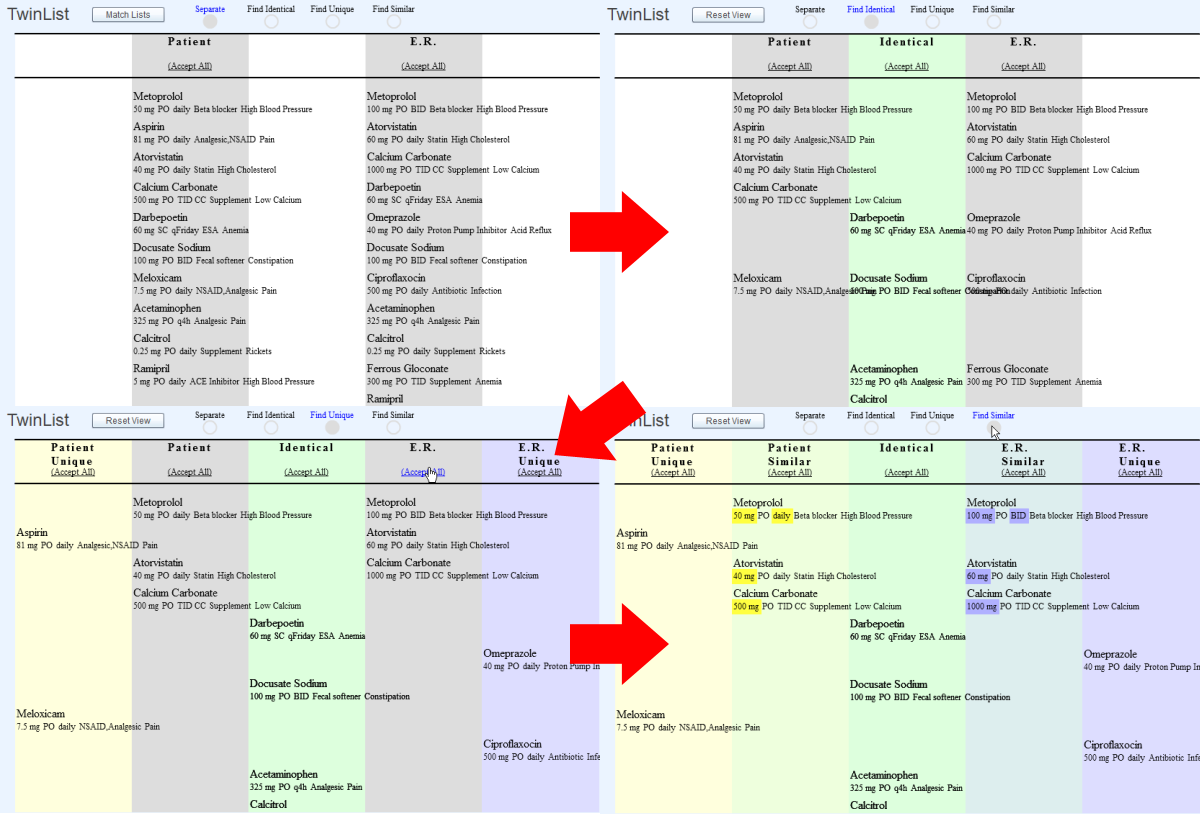
\includegraphics[width=1\linewidth]{img/anim_arrows.png}
\end{center}
   \caption{An animation sequence matching two lists of prescription drugs. The original \ListViewer~ is shown at the top left. In the top right, the \Identical~ items were found. The \Unique~ items are found next in the bottom left view. Finally, the \Similar~ items are matched with their differences highlighted in the bottom right view.}
   \label{fig:animation}
\end{figure*}

\subsection{Controls}
The \Controls, depicted in Figure~\ref{fig:controls}, contains functionality for organizing and manipulating the the \ListViewer~ visualization. This includes the following components:
\begin{itemize}
\item \SizeBy: scales item text by its value for the given attribute. This control only works with numerical-type attributes.
\item \ColorBy: colors item text by its value for the given categorical attribute. This control only works with categorical-type attributes.
\item \GroupBy: organizes items by their values for the given attribute. This control works with either categorical- or general-type attributes (but not numerical).
\item \SortBy: sorts items (within groupings) by their values for the given attribute. This control works with any attribute. Note that the \GroupBy~ control has precedence over this control.
\end{itemize}
As of the submission of this paper, the \SizeBy~ and \ColorBy~ functionality is not operational, due to time constraints, though these features are planned for future iterations.

For an example of the usefulness of these features, consider the following scenario in the context of analyzing the State of the Union addresses. One might begin by grouping items (words) by their part of speech (assuming part of speech is an attribute). To further organize the display, one might then sort items by name (i.e. alphabetical ordering). The former lets the user analyze syntactical patterns, while the latter enables quick lookup of particular keywords. One can go even further, sizing words by their TF-IDF value, to reveal lexical patterns, similar to a Wordle\cite{Viegas2009}. In the context of medication list reconciliation, one might wish to group by drug class, size by dosage and color by frequency.
 
\begin{figure}
\begin{center}
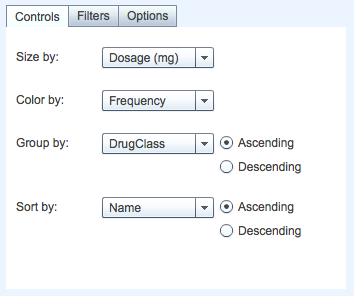
\includegraphics[width=1\linewidth]{img/controls.png}
\end{center}
   \caption{A detail of the \Controls.}
   \label{fig:controls}
\end{figure}

\subsection{Filters}
\TwinList's \Filters~ were inspired by those of Spotfire\cite{Ahlberg1996}. The ability to perform realtime queries and see the changes propagate to the visualization augments data exploration and analysis. For example, in medication list reconciliation, one might wish to display only certain drug classes, or only dosages in excess of a certain amount.\footnote{While in practice dosages are typically given on multiple scales --- e.g. 325 mg, 30 CCs --- we require that all numerical attribute values be normalized to the same scale.} Figure~\ref{fig:filters} depicts a detail of the \Filters.

Filters come in two classes: categorical and numerical. Categorical filters can be used to display only a specific set of attribute values, taken from a finite set of possible values. Numerical filters can be used to display only attribute values that fall within specified lower and upper bounds. Note that an item will only display it passes all filters, meaning its attribute values fall within the specified allowable sets or ranges.

A filter can be enabled and disabled via a checkbox displayed to the right of it. Enabling a filter implies that it is active. When a filter is disabled, it has no effect on the \ListViewer, no matter which values or bounds are set. The \textit{Select All} and \textit{Clear All} buttons select or deselect all options in a categorical filter, where selection is demarcated by highlighting. A selected value is kept in the visualization. In a numerical filter, both \textit{Select All} and \textit{Clear All} simply reset the bounds.

\begin{figure}
\begin{center}
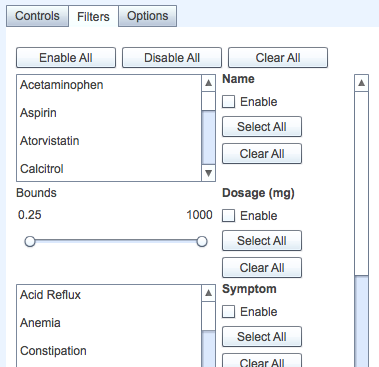
\includegraphics[width=1\linewidth]{img/filters.png}
\end{center}
   \caption{A detail of the \Filters.}
   \label{fig:filters}
\end{figure}

\subsection{Options}
The \Options~ allows the user to control the following global application behavior:
\begin{itemize}
\item \textit{Dataset}: selects and loads a dataset from the three demo sets.\footnote{In future versions, the user will be allowed to upload a dataset using our proprietary XML schema.} Upon changing the dataset, the application will be reset, except for the \Options.
\item \textit{Font size}: sets the size of the font used to display item names in the \ListViewer. Note that the attribute text font size is relative to that of the name, though slightly smaller to reduce clutter.
\item \textit{Animation speed}: controls the relative speed of the animations in the \ListViewer. The speedup is defined as $2^\alpha$, where $\alpha$ is the slider value. Thus, a value of $\alpha = +1$ will double the speed and a value of $\alpha = -1$ will reduce it by $1/2$.
\item \textit{Link identical items}: determines how identical items are treated in the \ListViewer. When linked (the default), highlighting affects both items and accepting/rejecting either will hide the other from the \ListViewer. When unlinked, they are considered completely separate items.\footnote{Unlinking identical items implies that both items can be accepted or rejected, independent of the other.}
\item \textit{After item accept/reject}: determines the behavior of the \ListViewer~ after accepting or rejecting an item. \textit{Gray out} will simply gray the text and disable mouse actions; \textit{Remove} will hide the item from the \ListViewer.
\end{itemize}

\begin{figure}
\begin{center}
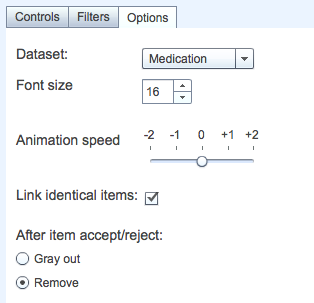
\includegraphics[width=1\linewidth]{img/options.png}
\end{center}
   \caption{A detail of the \Options.}
   \label{fig:options}
\end{figure}

\section{Evaluation}
Our goal was to deliver a working prototype, not a finished, fully-functional application. As such, we are more concerned with qualitative than quantitative feedback on the features of our visualization system at this point. According to the categorization proposed by Lam et al~\cite{lam-bertini-isenberg-plaisant-carpendale-2011}, the evaluation scenario best matching our present purposes is the \textit{User Experience (UE)} test case. The goal of the following experiments is to observe how users react to the visualization and interaction features offered by \TwinList. We will use their feedback to improve the system's design in future versions.

\subsection{Experiment Design}
Our test subjects came from two populations: two physicians and two non-specialist participants. The former used \TwinList to perform medication reconciliation; The testing protocol proceeded as follows: first, the user watched a $~7$-minute video demonstrating basic usage. Following this, the user was allowed to ask questions. Next, the user interacted with the system unaided, performing either specific tasks (medication reconciliation case studies). While using the system, subjects were encouraged to \textit{think aloud}~\cite{lewis-1982}. The entire experiment was captured in both audio and screen capture video. 

For the latter population, we used the car features data set for the evaluation. The data set consists two lists of car features for two different type of cars. It is a good supplement for the medication data because it's more familiar to the general public, in this case, students. Also, we are using the State-Of-The-Union(SOTU) bag-of-words data. It contains two lists of words used in the SOTU speech of Bush and Obama. The data size is huge, so we filtered the data and only keep the most frequent-using words. The testing protocol proceeded as follows: at first, we explain the concept and some basic usage. Then, we asked the participants to explore the interface themselves. If they raised questions, we will explain to them. Then we asked them to perform two tasks on the car features data to test the learnability and usability of the interface. At last, we asked them to explore the SOTU data to see if the visualization is enough for them to find insights. During the test, they are also encouraged to \textit{think aloud}.

\subsection{Case 1: Med. reconciliation, A. Z. H., male, 34 y. o.}
Overall, the participant performed the tasks as expected and reported anticipated results. A. Z. H. purported to be very comfortable with computers. He does not perform medication reconciliation on a regular basis, except when doing inpatient aid and discharge from the hospital, for which he does not use any software. This is how he describes his \TwinList~ experience: \textit{``It's really impressive, the way you organize things is great. It's definitely a step in the right direction \dots"}. He was very enthusiastic and provided several suggestions, most of all worth including in this section. 

\subsubsection{Results}
This is our reading of A. Z. H.'s experience:
\begin{itemize}
\item There is need for an indication that there are more items than what can be currently seen in a column. The scroll bar alone is insufficient.
\item It is difficult to get to the \AcceptReject~ pop-up menu when accepting/rejecting an item. He had trouble with the click-and-hold behavior, wanting instead to use the mouse's right-click button.
\item To send items from \AcceptedRejected~ lists back to the viewer one-by-one requires quite some effort when you have many items in those lists. A \textit{Remove All} button would be desirable.
\item Warning dialogs or undo may be needed when accepting and rejecting items, since it is a delicate operation in medication reconciliation.
\item In the control panel, drop-down boxes should indicate what the default \GroupBy/\SortBy~ attributes are, instead of blank captions. (The default is actually the original ordering.)
\item It would be desirable to shorten vertical empty spaces in between items to minimize the need of scrolling.
\item The number of visible item attributes should be shortened in the \ListViewer, since reconciliation is performed, in practice, based on only a few (e. g. the \textit{Indication} feature).
\item For items in the \Similar~ columns, the item pop-up menu should have a third option, to automatically reject an item of a list if its counterpart at the other list was accepted. According to the participant, this would be the likely outcome in almost every such context.
\item The participant suggested that we should change the way items are displayed so that, for each list, you have items sorted by some \textit{uniqueness level}; for example, by vertically ranging from identical to unique. This would add more meaning to the vertical structure of the list, which is somewhat lost after lists are matched, but would represent a significant change in the concept.
\item The participant felt that placing the \AcceptedRejected~ lists at the bottom of the interface may be suboptimal for tracking what happened to processed items, especially when the user gets distracted.
\item The participant missed being able to interact on the spot with accepted/rejected items that are grayed out. In his words: \textit{``If it is grayed out, what if (\dots) I really want to do the 100 mg, is there any way to click and have it re-instate (\dots) or un-reject/un-accept"}. He believes that if he could interact with grayed-out items on the viewer, the \AcceptedRejected~ lists might not even be necessary, thus allowing more room for the main visualization. As such, the list of rejected/accepted items could be output as the final product of the interactive process and would be activated by pressing a button. As he suggested: \textit{``\dots Here is your final list of medications, this is your rejected list over here, and when one finally accepts, export to (\dots) or put in patient's medical record \dots"}.
\item The participant suggested an additional \SortBy~ criteria: in his own words, \textit{``medications that haven't been dealt with yet."} We translate this as a grouping of medications based on their accepted/rejected status. This is a useful, general concept applicable to other list matching problems.
\item The participant mentioned the importance of filters, especially to filter by route (e.g. I.V. medications).  
\end{itemize}

\subsection{Case 2: Med. reconciliation, M. G., male, 62 y. o.}

As opposed to the previous participant, M. G. had more trouble to perform his tasks. It was clear from his reactions that he was expecting the system's terminology to be more towards medication reconciliation (such as having \textit{Match Lists} as the caption of the button that triggers list matching, instead of \textit{Reconcile Lists}) than general list matching. As the matching animation began, he clearly expressed a feeling of overwhelm: \textit{``Wow, what just happened there?"}. M. G. considers computers somewhat hard to use (he reported a difficulty score of 4 out 5). This subject does medication reconciliation every day. 
\subsubsection{Results}
This is the summary of M. G.'s results:
\begin{itemize}
\item In his opinion, one item's list of attributes should not exceed the width of its column. He felt that the piece of the attribute list that slops over to the next column could be associated with another item in that column, which could lead to a serious confusion: for example, the dosage of one medication could be associated with another by mistake, as he pointed out himself. 
\item The user got confused by the step-wise animation buttons when told to accept all identical items. He clicked at \textit{Find Identical} instead of \textit{Accept All} at the \Identical~ column of the viewer, when told to accept all identical items. The animation then went half-way through and he realized he did not do what was expected. He then tried to fix it and ended up clicking on \textit{Find Unique}. Finally, when he tried to accept/reject items, he realized that similar items across both lists were not in the same row of the viewer. The reason was that he did not perform the list matching all the way, \textbf{a sign that list matching should be performed as an atomic operation}. That is also supported by the fact that the first physician has not even touched the step-wise matching feature.
\item An unexpected outcome of this test was that the user somewhat associated temporal order from left to right, as if the first list represented an event that necessarily came before the second list. He compared the dosage of the drugs at the Patient's \Similar column (left) with the corresponding drugs/dosages at the E.R. column (right), and tried to infer some sort of temporal pattern regarding how the patient was dealt with in emergency: \textit{``Conceptually, I think it is a nice setup, actually. Because you can try to deduce what went on during the stay in the E. R. For these drugs, they decided that the patient needed more of that, because they increased the dose ..."}. Although this was not intended when the lists were fed to the system or however the data were displayed, to associate temporal meaning to lists might be an interesting path to explore in the future.
\item The issue of having to unnecessarily reject a similar item after accepting its counterpart appeared again, particularly if dosage is the single attribute that changed across items: \textit{``If it is absolutely the same in every respect, except for the dosage amounts, you can't give two dosage amounts simultaneously ..."}.
\item Different from the other participant physician, M. G.  thinks \textit{Indication} is not a very descriptive attribute since a drug can be prescribed for several reasons. On the other hand, he likes the \textit{Drug Class} feature and, after being asked about it, he agrees it could be a useful feature to group by.
\end{itemize}


\subsection{Case 3: General Data, T. L., male.}
The participate is a computer science Ph.D student focus his study on Human Computer Interaction. He obtained his M.S. degree in design of interaction and he has many design and evaluation experience. He did not grasp the concept of the medication reconciliation immediately at the beginning. But after we explain and provided background information, he understood the concept well. He performed the tasks very well with few problem or difficulties. He was very pleased by the matching animation, he expressed "I really like the animation effect". 
\subsubsection{Results}
This is the summary of the experiment results:
\begin{itemize}

\item He suggested that the screen space is not enough for the visualization and we should utilize the screen space more efficiently.

\item During the test, he used the stepped animation a lot, instead of the "match list" button on the left. It suggested that the steps of the animation might be useful to help user understand the animation steps, but the wording of the label should be changed. Also, make the steps non-clickable seems to be another good option. 

\item After he explored both car feature data and SOTU data, he stated that the accept/reject actions did not make sense when used for general data sets. He spend some time viewing the SOTU data visualization, and he didn't find much interesting insights. He suggested that it would be better if we can provide contextual information about the words. 
\end{itemize}



\subsection{Case 4: General Data, A.N.S., female.}
The participate is a computer science Ph.D student focus her study on Human Computer Interaction. The overall testing experiment went very well. She had no problem interpret the visualization. For all the tasks, she immediately came up the plan on how to find the similarity and difference of the two lists and described her action clearly. The only difficulty she encountered is the operation to add list item to the action list, but after she is reminded with the correct operation, she had no problem with taking actions. She stated "nice visualization" at the end of the evaluation.
\subsubsection{Results}
The following is the summary of the experiment results:
\begin{itemize}
\item The only difficulty she encountered is the operation to add list item to the action list, but after she is reminded with the correct operation, she had no problem with taking actions afterwards.

\item When she was exploring the filters, she was confused by the options shown in the drop down menu, especially the "group by" option  "priority ()". She said it looked like a function rather than the name of one of the attributes. She suggested that we should use more understandable wording for the attributes when we preprocessing the data. 
\item She really liked the filters and the idea of be able to filter the data, She said "so cool, I love this" after she saw the filtering result. However, what she did not like the size changing of the colored background after she performed filtering. 

\end{itemize}


\section{Conclusions and Further Directions}


From the medication reconciliation results, we can say that both users approved the idea of having the items of the two lists organized according to five levels of similarity, one of the main concepts behind \TwinList. They also emphasized the importance of the highlighting (attribute-based differences) feature and proposed that the list of attributes should be shortened and limited to a few key properties more commonly employed in medication reconciliation, such as \textit{Indication}, \textit{Drug Class} or \textit{Route}.

We also learned that the step-wise list matching feature appears to be superflous and potentially troubling. The first physician did not use the feature, and the second was seriously confused by it. This suggests that list matching both from the procedural and animation perspective, should be performed atomically. 

Another lesson was that the acceptance of an item in the \Similar~ column of one list will almost always imply the rejection of the other list's corresponding item (and vice-versa), therefore a third option that accepts one item and reject its counterpart appears to be desirable in the context of medication reconciliation. Other interesting conceptual ideas as well as small interface changes were discussed, as detailed in the previous section.



\bibliographystyle{abbrv}
\bibliography{twinlist}

\end{document}
